\chapter{Implementation}

\section{Implementation of covert modules}
\label{sec:impl_cov_mod}

The following is an extract from the source code of the framework (\url{FaucetEnv/Faucet/src/covert_channels/covert_channels.jl}) that shows the implementation of a covert module.

\begin{lstlisting}[language=JuliaLocal, style=julia]
ipv4_identifaction::covert_method{:IPv4_Identification} = covert_method(
    "IPv4_Identification",
    Layer_type(3), # network
    "IPv4_header",
    8,
    16, # 2 bytes / packet
)

# Init function for IPv4_Identification
function init(::covert_method{:IPv4_Identification}, net_env::Dict{Symbol, Any})::Dict{Symbol, Any}
    target_mac, target_ip = net_env[:dest_first_hop_mac], net_env[:dest_ip].host
    return Dict{Symbol, Any}(
        :payload => Vector{UInt8}("Covert packet!"), # not a real payload
        :env => net_env,
        :network_type => IPv4::Network_Type,
        :transport_type => TCP::Transport_Type,
        :EtherKWargs => Dict{Symbol, Any}(
            :dest_mac => target_mac,
        ),
        :NetworkKwargs => Dict{Symbol, Any}(
            :dest_ip => target_ip,
        )
    )
end

# Encode function for IPv4_Identification
function encode(::covert_method{:IPv4_Identification}, payload::UInt16; template::Dict{Symbol, Any})::Dict{Symbol, Any}
    template[:NetworkKwargs][:identification] = payload
    return template
end
encode(m::covert_method{:IPv4_Identification}, payload::String; template::Dict{Symbol, Any})::Dict{Symbol, Any} = encode(m, parse(UInt16, payload, base=2); template=template)

# Decode function for IPv4_Identification
decode(::covert_method{:IPv4_Identification}, pkt::Packet)::UInt16 = pkt.payload.payload.header.id
\end{lstlisting}

This implementation makes use of Julia's multiple dispatch system, allowing for different functions to be called depending on the type of arguments. The three defined functions \inline{init}, \inline{encode}, and \inline{decode} are called with the covert channel as the first argument.

I designed the covert channels to be a composite parametric type, where the type parameter is the type of channel, this prevents ambiguity when the multiple dispatch system is used. The parametric type definition looks like this:

\begin{lstlisting}[language=JuliaLocal, style=julia]
struct covert_method{Symbol}
    name::String
    layer::Layer_type
    type::String # What packet type are we aiming for?
    covertness::Int8 # 1 - 10
    payload_size::Int64 # bits / packet
    covert_method(name::String, layer::Layer_type, type::String, 
    
    covertness::Int64, payload_size::Int64)::covert_method{Symbol} = new{Symbol(name)}(name, layer, type, Int8(covertness), payload_size)
end
\end{lstlisting}

This struct instantiation implicitly converts the name of the covert channel to a symbol, which is used as the type parameter.

\section{Algorithm implementation}
\label{sec:algorithm_impl}

The input variables and output of the implementation can be found in \fullref{sec:decision_algorithm}. This section will cover the entire algorithm, getting from the input variables to the output.

This function is written in Julia, making use of its ability to use Unicode characters in variable names, allowing me to use the same mathematical notation in the code as in the design documentation. The following is an extract from the source code of the framework (\url{FaucetEnv/Facuet/src/covert_channels/covert_channels.jl})

\begin{lstlisting}[language=JuliaLocal, style=julia]
function method_calculations(covert_methods::Vector{covert_method}, env::Dict{Symbol, Any}, Eₚ::Vector{Int64}=[], current_method::Int64=0)::NTuple{2, Vector{Float64}}
    # Get the queue data
    q = get_queue_data(env[:queue])

    # Covert score, higher is better : Method i score = scores[i]
    S = zeros(Float64, length(covert_methods))
    # Rate at which to send covert packets : Method i rate = rates[i]
    R = zeros(Float64, length(covert_methods))
    
    if isempty(q)
        @error "No packets in queue, cannot determine method" q
        return S, R
    end
    
    #@warn "Hardcoded response to determine_method"
    L = [get_layer_stats(q, Layer_type(i)) for i ∈ 2:4]

    # Eₗ : Environment length : Number of packets in queue
    Eₗ = length(q)

    # Eᵣ : Environment rate : (Packets / second)
    Eᵣ = Eₗ / abs(last(q).cap_header.timestamp - first(q).cap_header.timestamp)

    # Eₛ : Environment desired secrecy : User supplied (Default: 5)
    Eₛ = env[:desired_secrecy]

    # Get the count of hosts local to the supplied ip (we don't want to consider external ones).
    Eₕ = get_local_host_count(q, env[:dest_ip])

    for (i, method) ∈ enumerate(covert_methods)
        Lᵢ_temp = filter(x -> method.type ∈ keys(x), L)
        if isempty(Lᵢ_temp)
            @warn "No packets with valid headers" method.type L
            continue
        end
        # Lᵢ : the layer that method i exists on
        Lᵢ = Lᵢ_temp[1]

        # Lₛ : The sum of packets that have a valid header in Lᵢ
        Lₛ = +(collect(values(Lᵢ))...)

        # Lₚ : Percentage of total traffic that this layer makes up
        Lₚ = Lₛ / Eₗ

        # Pᵢ is the percentage of traffic 
        Pᵢ = Lₚ * (Lᵢ[method.type] / Lₛ)

        # Bᵢ is the bit capacity of method i
        Bᵢ = method.payload_size

        # Cᵢ is the penalty / bonus for the covertness
        #  has bounds [0, 2] -> 0% to 200% (± 100%)
        Cᵢ = 1 - ((method.covertness - Eₛ) / 10)

        # Score for method i
        #  Pᵢ * Bᵢ : Covert bits / Environment bits
        #  then weight by covertness
        #@info "S[i]" Pᵢ Bᵢ Cᵢ Pᵢ * Bᵢ * Cᵢ
        S[i] = Pᵢ * Bᵢ * Cᵢ

        # Rate for method i
        #  Eᵣ * Pᵢ : Usable header packets / second
        #  If we used this much it would be +100% of the environment rate, so we scale it down
        #  by dividing by hosts on the network, Eₕ.
        #  then weight by covertness
        #  We don't want to go over the environment rate, so reshape covertness is between [0, 1] (1 being 100% of env rate)
        #  (Eᵣ * Pᵢ * (Cᵢ / 2)) / Eₕ : Rate of covert packets / second
        #  ∴ 1 / Eᵣ * Pᵢ * (Cᵢ / 2) : Interval between covert packets
        #@info "R[i]" Eₕ Eᵣ Pᵢ Cᵢ/2 Eₕ / (Eᵣ * Pᵢ * (Cᵢ / 2))
        R[i] = Eₕ  / (Eᵣ * Pᵢ * (Cᵢ / 2)) 
    end

    # Eₚ (arg) : Environment penalty : Penalty for failing to work previously
    for i ∈ Eₚ
        S[i] *= 0.1 # 10% of original score
    end

    # Allow for no current method (as the case is when recovering)
    current_method != 0 && (S[current_method] *= 1.1) # Encourage current method (+10%)

    return S, R
end
\end{lstlisting}

The \inline{method\_calculations} function only does the calculations, not the selection of the best method, which is done by a function that wraps this one and returns an index $i$ and a rate $R_i$ for the highest scoring method ($S_i$).

\section{Integrity check}
\label{sec:integrity_impl}

The integrity check process has two main parts, the sender, and the receiver. For both of the processes, the integrity is calculated using the same function (\url{FaucetEnv/Facuet/src/utils.jl}):

\begin{figure}[h]
\begin{lstlisting}[language=JuliaLocal, style=julia]
function integrity_check(chunk::String)::UInt8
    padding = 8 - (length(chunk) % 8)
    # Payload may not be byte aligned, so pad it
    chunk *= padding == 8 ? "" : "0"^padding
    return crc(CRC_8)([parse(UInt8, chunk[i:i+7], base=2) for i in 1:8:length(chunk)])
end
\end{lstlisting}
\caption{\inline{integrity\_check} function}
\end{figure}

This function uses a CRC8 checksum, but in reality, its implementation is not important, the only requirements are that the function is deterministic and that a single byte is returned. A consideration for choosing such a function should be its behaviour when there is not a guarantee that the current chunk is a multiple of 8 bits, as discussed in \fullref{sec:mp_consequence}, if the checksum function requires bytes, then the chunk must be padded in a deterministic way.

To prevent inconsistencies in the check, the same function is used by both the sender and receiver, by putting the function in the shared \inline{utils.jl} file.

The sender needs to issue the challenge and receive the response. The challenge piggybacks the method change protocol, so it just needs to await the response from the receiver. It does this by opening a raw socket and listening for an arp packet from the target to the known host it used to create the offset. We can see the challenge and response process in the \inline{send\_covert\_payload} function (found in \url{FaucetEnv/Facuet/src/outbound/packets.jl}) in figure \ref{fig:chal_resp}.

\begin{figure}[h]
\begin{lstlisting}[language=JuliaLocal, style=julia]
# Get the current integrity, if we have used final padding, append it
integrity = integrity_check(bits[chunk_pointer:pointer-1] * final_padding)
# Get a known host for the integrity check
known_host = get_local_net_host(net_env[:queue], net_env[:src_ip], host_blacklist)
# Send the challenge
send_method_change_packet(method, method_index, integrity ⊻ known_host, net_env, method_kwargs)

...


# Await the response
if await_arp_beacon(net_env[:dest_ip], known_host, check_timeout) # Success
    # reset failures
    protocol_failures = 0
    @debug "Integrity check passed" method=method.name integrity known_host integrity ⊻ known_host
    # reset chunk pointer
    chunk_pointer = pointer
    # update last verified integrity (+ length)
    last_integrity = (chunk_pointer, integrity)
else
    ...
\end{lstlisting}
\caption{Challenge and response process implementation}
\label{fig:chal_resp}
\end{figure}

Once the packet is sent, the sender enters the \inline{await\_arp\_beacon} function, providing the IP address of the target (which we expect the source of the ARP request to be), the known host (which we extract from the local network (line 4), as discussed in \fullref{sec:improving_arp}), and a timeout of how long to wait, in seconds. The timeout is largely unimportant as the function will return as soon as it receives the expected packet, which is normally a fraction of a second. The function can be seen in figure \ref{fig:await_arp_beacon}.

\begin{figure}[h]
\begin{lstlisting}[language=JuliaLocal, style=julia]
    function await_arp_beacon(ip::IPv4Addr, target::UInt8, timeout::Int64=5)
    # Get a fresh socket to listen on
    socket = get_socket(AF_PACKET, SOCK_RAW, ETH_P_ALL)
    start = time_ns()
    while (time_ns() - start) < timeout * 1e9
        # Read a packet
        raw = read(socket)
        # Confirm it is more than the minimum size of an ARP packet
        if length(raw) >= 42
            # Check it matches our boilerplate ARP
            if raw[ARP_SEQUENCE_SLICE] == ARP_SEQUENCE
                # Check it is from the source we are looking for
                if raw[ARP_SRC_SLICE] == _to_bytes(ip.host)
                    # Check it is to the target we are looking for
                    if raw[ARP_DEST_SLICE][4] == target
                        return true
                    end
                    push!(heard, raw[ARP_DEST_SLICE][4])
                end
            end
        end
    end
    return false
end
\end{lstlisting}
\caption{\inline{await\_arp\_beacon} function}
\label{fig:await_arp_beacon}
\end{figure}

\subsection{Final integrity check}

An oversight of the integrity process outlined in the \fullref{sec:integrity} section is the last chunk does not get verified, this undermines the entire integrity of the entire process, the solution was to add a final integrity check. Because of the design of the packet-sending function, a loop that iterates the payload, verifying the last chunk of data becomes less trivial, as we want to perform the check after the loop, but if the check fails we would have to return to the loop, this would require a confusing nested loop structure and would be difficult to read, especially when the already complex function is considered. To solve this problem, I utilised the \inline{@goto} and \inline{@label} macros provided by Julia, this creates an unconditional jump to a label, allowing me to jump back to the integrity check when combined with a flag \inline{finished} that indicates there is no more data to send if the integrity check succeeds with the flag set, it will break the loop, otherwise, it will resend the chunk as usual.

This worked, however, the final integrity check always failed. The reason for this was the sender was creating the integrity check using the payload, but the receiver was creating the integrity check using the payload and the padding, meaning that despite the data being the same, the integrity check was different. To solve this problem, I added a variable \inline{final\_padding} (see line 2 of figure \ref{fig:chal_resp}) that is an empty string unless it is the final chunk, in which case it is the padding added to the payload to fill the channel capacity. 

The implementation of this is spread across the entire \inline{send\_covert\_packet} function and thus is difficult to show in a code snippet, but it can be seen in the source code (\url{FaucetEnv/Facuet/src/outbound/packets.jl}).

\section{Getting a valid TCP server}

For the TCP Acknowledgement bounce channel I wanted to use a locally accessible TCP server to showcase how the framework allows adaption to the environment at a channel level, As discussed in \fullref{sec:covert_modules}. Unfortunately, because my test environment is a packet capture replay, the server found by the framework cannot be communicated with (as there is no host to communicate with). To solve this problem, I hardcoded the response to point at a valid server, this is not ideal, but it is a workaround for this project. We can still see the server that the framework finds in the packet capture.

\begin{figure}[h]
    \centering
    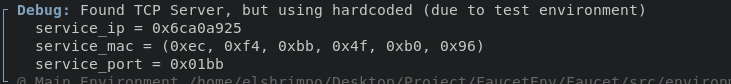
\includegraphics[width=0.5\textwidth]{fig/GET_TCP_debug.png}
    \caption{The TCP server found by the framework}
    \label{fig:tcp_server}
\end{figure}

\begin{figure}[h]
    \centering
    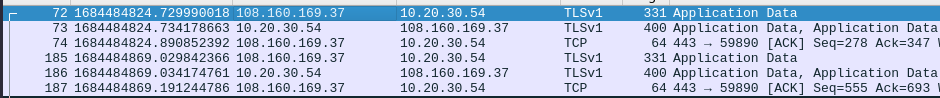
\includegraphics[width=0.5\textwidth]{fig/GET_TCP_pcap.png}
    \caption{The TCP server found by the framework in the packet capture}
    \label{fig:tcp_server_pcap}
\end{figure}

The \inline{get\_tcp\_server} function works by looking at the TCP traffic in the environment, It favours traffic that is going to, or from, a TCP service like HTTP (Port 80) or HTTPS (Port 443). If it cannot find any of those it will simply look for a TCP packet with the SYN Flag set, which indicated a server, and then return it.

\begin{lstlisting}[language=JuliaLocal, style=julia]
function get_tcp_server(q::Vector{Packet})::Union{Tuple{NTuple{6, UInt8}, UInt32, UInt16}, NTuple{3, Nothing}}
    common_query = Vector{Dict{String, Dict{Symbol, Any}}}([
        Dict{String, Dict{Symbol, Any}}(
            "TCP_header" => Dict{Symbol, Any}(
                :dport => TCP_SERVICES
            )
        )
    ])
    # Clients connected to common TCP Services, TCP traffic to them is favourable (In terms of covertness)
    services = query_queue(q, common_query)
    
    ...

    service_mac, service_ip, service_port = nothing, nothing, nothing
    if !isempty(services)
        # Take the most recently active one
        service = pop!(services)
        # This is a packet going toward tcp service
        service_mac = getfield(service[layer2index["Ethernet_header"]], :source)
        # Ethernet_header -> tcp server mac (of next hop from local perspective)
        service_ip = getfield(service[layer2index["IPv4_header"]], :daddr)
        # IP_header.daddr -> tcp server ip
        service_port = getfield(service[layer2index["TCP_header"]], :dport)
        # TCP_header.dport -> tcp server port
    else
    ...
    return (mac, ip, port)
end
get_tcp_server(q::CircularChannel{Packet})::Union{Tuple{NTuple{6, UInt8}, UInt32, UInt16}, NTuple{3, Nothing}} = get_tcp_server(get_queue_data(q))
\end{lstlisting}

